\documentclass[titlepage,a4paper, fleqn, flalign]{article} \usepackage[pdftex]{graphicx}
\usepackage[multiple]{footmisc} \pagestyle{myheadings}
\usepackage[latin1]{inputenc}
\usepackage{fancyhdr}
\usepackage{rotating}
\usepackage{graphicx}
\usepackage{longtable}
\usepackage{amsmath}
\usepackage{ltxtable}
\usepackage{tabularx}
\usepackage{rotating}
\usepackage{array}
\usepackage{amssymb}
\usepackage{pstricks}
\usepackage{qtree}
\usepackage{lscape}
\usepackage{setspace}
\usepackage[numbers,round]{natbib}
\usepackage{harvard}

\graphicspath{{Figures/}}


\begin{document}


%\title{Draft  \\[2cm]
%\textbf{Structural Breaks in Inflation Rates}}
%
%\author{ \scriptsize by \\
%Mag. Thomas WINDBERGER\\
%Prof. Dr. Achim ZEILEIS \\
%\scriptsize Doctoral Advisors: \\
%\scriptsize Univ.-Prof.Dr. Jesus Crespo-Cuaresma \\
%\scriptsize A.Univ.-Prof.Dr. Janette Walde \\ [1cm]}
%
%
%
%\maketitle

% anderthalb Zeilen Abstand inne


\setstretch{1,5}


\section{Abstract}

The aim of this paper is to shed some light on the effect of the European Monetary Union (EMU)  on changing the volatility of the inflation rates in its Member States. 
%We concentrate on the volatility of the inflation rate rather than its mean since \cite{fried} conjectured that the harmful effect of inflation on growth is driven by inflation volatility. 




\newpage
\section{Introduction}

The ECB defines price stability ``as a year-on-year increase in the Harmonised Index of Consumer Prices (HICP) for the euro area of below 2 \%'' \cite{castel}. \cite{emerson} makes it clear, that a high inflation rate is also more variable and uncertain and in that way causes more relative price variability, leading to a less efficient price mechanism (p.~22). Thus to achieve a low inflation rate and low variability of inflation must be a key issue for the central bank. \\
To further justify the use of inflation volatility, we refer to \cite{rother}: ``Among the harmful effects of inflation, the negative consequences of inflation volatility are of particular concern. High variability of inflation over time makes expectations over the future price level more uncertain. In a world with nominal contracts, this induces risk premia for long-term arrangements, raises costs for hedging against inflation risks and leads to unanticipated redistribution of wealth. Thus, inflation volatility can impede growth even if inflation on average remains restrained.'' \\
The question of interest centers around the way in which a countries decision to join the EMU changed its inflation volatility. There are a number of reasons why the volatility of  one of these nations should change indeed. Given that the country experienced quite volatile inflation rates, its efforts to meet the convergence criterias are likely to lead to a change in the volatility of their respective inflation rates, as has indeed been the case for a number of EMU countries, like Spain, Portugal, Italy and Greece. 


\section{Literature Overview}


%Sinn: Zusammenfassung der gegebenen Literatur. Darstellen, was in der Richtung publiziert wurde und herausarbeiten, warum mein Ansatz hier jetzt neu sein soll und warum die Frage noch nicht beantwortet ist.

Theory unfortunately is quite unsure about whether or not the creation of a monetary union between two or more states is likely to reduce/increase the variability or even the level of the inflation rate.  \cite{cooper} points out, that "a central bank under a monetary union will internalize the interdependence between countries and optimally choose a lower inflation rate" and he argues that a "central Bank governing the growth of money supply will optimally choose zero inflation." This is not the case with the ECB which targets at 2\% so as to avoid the risk of deflation. It is thus not quite clear how a monetary union will affect the volatility and the level of the inflation rate.\\
An interesting approach to this question is taken by \cite{holte}. He creates a two country model for monetary policy analysis along the line of two models by \cite{mc1} and \cite{mc2} as well as \cite{gali}. The inflation is modeled by a hybrid Phillips curve (NKPC) specification and there are a number of different home country interest rate rules, like strict inflation targeting, flexible targeting, pegging to a currency and --  monetary union. What he finds out via simulations of these different interest rate rules is that the standard deviation of the home CPI inflation rate can be substantially reduced by joining a monetary union. But monetary policy in a monetary union does not explicitly stabilize the output gap and inflation rate in case of national economic shocks. The effects of joining on inflation rate variability depend on structural parameters like risk aversion, price flexibility, export demand elasticity, openness and shock correlations. Due to the fact that not all of these parameters are known and that their interaction as well has to be guessed, theory has some troubles answering the question of this paper. \\
\cite{cap} estimate short-run and steady-state inflation uncertainty in 12 EMU countries and find a considerable degree of heterogeneity across EMU countries in terms of average inflation, its degree of persistence and both types of uncertainty. They use a time-varying model with a GARCH specification for the unconditional volatility of inflation and find some instability in the conditional volatility. \\
In a paper examining structural convergence of the inflation rates in EU counries, \cite{sarno} try to answer the question if during the 1990s the inflation rate dynamics of EU countries become more similar. They find that convergence in time of inflation dynamics was only partly observeable. The same is also found by \cite{palomba}, they too find little evidence of similarity of short-run inflation dynamics. \\
In a paper studying core inflation and using an aggregated Euro Area inflation rate, \cite{morana} finds three regimes (roughly 1980-1984, 1984-1993 and 1993-2000) governing the core inflation rate.  \\
Inquiering into the convergence properties of inflation rates among countries of the EMU, \cite{busetti} find that from 1980-1997 there was convergence of inflation rates, but afterwards there is some diverging behavior. \\
%A otherwise very interesting paper by \cite{maheu} can not be used due to its defintion of a structural break as "`an unpredictable event in which the relationship among the variables in a model change"', which differs from the definition of a sructural break used in this paper.






\section{Data}

Inflation is measured as the logarithm of the monthly change in the HICP from 1.1990---3.2010, so $x_t = 100\cdot ln(HICP_{t}/HICP_{t-1})$. Countries included are Austria,	Belgium,	Czech Republic,	Denmark,	Finland,	France,	Germany,	Greece,	Hungary,	Ireland,	Italy,	Luxembourg,	Netherlands,	Poland,	Portugal,		Spain,	Sweden,		United Kingdom and the	Euro area.  The data are obtained from the OECD Statistics. \\
The countries can be divided into three different groups: the EMU countries (Portugal, Spain, Italy, Greece, France, Belgium, Netherlands, Germany, Austria, Ireland, Slovenia, Luxembourg and Finland), EU members without ERM~II (Exchange Rate Mechanism): United Kingdom, Sweden, Poland, Czech Republic, Hungary. Denmark stands on its own as a member of the EU and the ERM~II, but not yet a member of the EMU.


% slovenien statt slovakei?
% Deutschland: CPI statt HVPI
% vielleicht ein paar L�nder aus dem Sample entfernen: 
% slovakei, tschechien, ungarn, polen
% Nachschauen, wann in den jeweiligen L�ndern die Entscheidung getroffen wurde, den Euro einzuf�hren. --> viel zu aufwendig


%/*  1 = austria = 240
%    2 = belgien = 228 (erst ab 91)
%    3 = czechrepublic = 180 (erst ab 95)
%    4 = denmark = 240
%    5 = finland = 240
%    6 = france = 240
%    7 = germany = 180
%    8 = greece = 180
%    9 = hungary = 180
%    10 = iceland = 180
%    11 = ireland = 180
%    12 = italy = 240
%    13 = luxembourg = 180
%    14 = netherlands = 240
%    15 = poland = 168
%    16 = portugal = 240
%    17 = slovakei = 180
%    18 = spanien = 216
%    19 = schweden = 240
%    20 = uk = 239 (fehlt 12.2009)
%    21 = euroarea = 168
%*/
%
%/* CPI Daten von:
%    22 = Japan = 240
%    23 = Norway = 240
%    24 = Switzerland = 240
%    25 = USA = 240
%/*


\newpage
\section{Methodology}

\subsection{Using a generalized logistic distribution (GL)}

In econometric issues, the logistic distribution is often used in income distributions and growth models. Its use stems from the usefulness of its longer tails and its higher peak, which fits these problems somewhat better. The use of the generalized logistic distribution as we will use it in this paper is somewhat scarcer. \cite{won} use a GL distribution in an regressio model with autocorrelated errors and assumes that they follow a GL distribution rather than a Student's t-distribution, as to model the fact that oftentimes is leptokurtic and severely left or right skewed. A similar GL distribution is also used in \cite{tolikas} who analyse extreme risk and value--at--risk in the German stock market, allthough they don't use a shape parameter. Regarding inflation rates, the GL distribution is --to our best knowledge-- only used in relationship with expected inflation. \cite{batchelor} use a logistic distribution (not its generalization) to model the distribution of mean expected inflation rates. \\
As allready stated, we now apply the general framework, as developed in \cite{z08} to a more specific model, in this case by means of a GL distribution.Prior to that, we would like to give a short justification for our using of the GL distribution. Regarding the data at hand, it was not possible to use the already existing method developed in \cite{z07}, since allmost all inflation rates, with the noteable exception of Greece, are not normally distributed and clearly exhibit asymmetric properties. Therefore, a somewhat more flexibel distribution had to be used. We needed a distribution exhibiting rather strong kurtosis and the property to be both left and right skewed. To this end we use a generalization of the logistic distribution as defined in \cite{johnson}. Its probability density is given by:

\begin{eqnarray}
& & f(\pi | \theta, \sigma, \delta) = \frac{\frac{\delta}{\sigma}*\exp^{-\frac{\pi_i-\theta}{\sigma}}}{(1+\exp^{-\frac{\pi_i-\theta}{\sigma}})^{(\delta+1)}}
\end{eqnarray}

with location ($\theta$), scale ($\sigma$) and shape ($\delta$). For b=1 the distribution simplifies to the logistic distribution, for b$<$1 it is skewed to the left and for b$>$1 it is skewed to the right. The moments are given by:

\begin{eqnarray}
& & E(\pi_i) = \theta + \sigma (\gamma(\delta) - \gamma(1)) \\
& & Var(\pi_i)  = \sigma^2(\gamma'(\delta)+\gamma'(1)) \\
& & Skew(\pi_i) =  \frac{\gamma''(\delta)-\gamma''(1)}{(\gamma'(\delta)+\gamma'(1))^{3/2}}
\end{eqnarray}

where $\gamma()$ is the digamma function and its derivatives. \\
The log-likelihood is given by:

\begin{eqnarray}
& & l(\delta,\theta,\sigma, \pi) = ln(\delta) - ln(\sigma) - \frac{1}{\sigma} (\pi-\theta) - (\delta+1) ln(1+\exp^{-\frac{\pi-\theta}{\sigma}})
\end{eqnarray}

The resulting score function ($\psi()$) for the parameters (the derivatives of the log-likelihood) are given by:

\begin{eqnarray}
& & \psi(\pi_i,\delta) = \frac{\delta l(\delta,\theta,\sigma;\pi)}{\delta \delta} = \frac{1}{\delta} - ln(1+\exp^{-\frac{\pi-\theta}{\sigma}}) \\
& & \psi(\pi_i,\theta) = \frac{\delta l(\delta,\theta,\sigma;\pi)}{\delta \theta} = \frac{1}{\sigma} - (\delta+1)*\frac{\frac{1}{\sigma}\exp^{-\frac{\pi-\theta}{\sigma}}}{(1+\exp^{-\frac{\pi-\theta}{\sigma}})} 
\end{eqnarray}


\begin{equation}
\begin{split}
&& \psi(\pi_i,\sigma) = \frac{\delta l(\delta,\theta,\sigma;\pi)}{\delta \sigma} = -\frac{1}{\sigma} + \frac{1}{\sigma^2}(\pi-\theta) - (\delta+1) * \\
&& \quad \frac{\frac{1}{\sigma^2}(\pi-\theta)\exp^{-\frac{\pi-\theta}{\sigma}}}{(1+\exp^{-\frac{\pi-\theta}{\sigma}})}
\end{split}
\end{equation}


An enhancement to the allready existing R package "`strucchange"', which currently does not support a generalized logistic distribution (GL) is provided with this paper. The asymptotic testing theory still holds for this generalization. [Beweis] \\
The first part of the results we are going to present here, i.e. the tests and the graphical illustration of the empirical fluctuation process can be found in \cite{z07}. the second part of the results - the dating procedure and the illustration of the denisties fitted for the subsamples (divided by the breaks) - ca be found in \cite{z10}.

\subsection{Tests}

\subsubsection{Cramer-von Mises statistic - Nyblom Hansen Test}

We use the Cram�r von Mises type test as given in \cite{z07}. The test statistic is given by:

\begin{eqnarray}
& & \frac{1}{n} \sum_{i=1}^n \Vert efp(\frac{i}{n}) \Vert_2^2
\end{eqnarray}

i.e. first the $L_2$ norm is used to aggregate over the components and then the mean of the resulting aggregated process is used as the test statistic. This can also be shown graphically as developed in 
%[wann war die Erstpublikation der graphischen Methode?].


%\subsubsection{Kolmogorov-Smirnov Test}
%
%As a goodness of fit test, we use the Kolmogorov Smirnov Test for as given in \cite{massey}.

\subsection{Densities}

Another thing we wish to look at is the change in the moments of the distribution after a break occured and whether or not the subsample fit of the GL-distribution is prefereable to another. Allthough our interest centers on the variance of the respective inflation rate, skewness should not alltogether be ignored. If we  observe - for example - a change in skewness from positive to negative from one regime to another, we could conclude that now we will observe higher values in the inflation rate since it shifted.

\newpage
\subsection{Expected Results}

To give an idea what we would expect, we give a short overview over the history of the EMU. Following the Delors Plan with his 3 stages, we have: stage I (1990-1994), stage II (1995-1998) and stage III (1999-2002) which ended with the introduction of the Euro as legal tender. If the EMU had a significant effect upon inflation rate volatility we would expect to find a break either in the 90ies, reflecting the various waves of integration or after the introduction of the Euro due to the popular "`Teuro"' argument (i.e. the claim that the Euro lead to a significant increase in prices following the year of its introduction). [Teuro besser formulieren, gibt es daf�r einen internationalen Term?]

%
%Geschichte f�r Interpretation 
%- verwende Daten seit 1990
%- 1. Stufe (ab 1990) � Vorbereitung durch Liberalisierung Geld- und Kapitalverkehr
%- 2. Stufe (ab 1994) � Konvergenz:
%- 3. Stufe (ab 1998) � �bergang zum Euro:
%- Euro W�hrung Buchgeld seit 1.1.1999
%- Euro W�hrung Bargeld seit 1.1.2002?

\section{Results}

The results presented here are for the countries within the Euro--zone (Austria, Belgium, Finland, France, Germany, Greece, Ireland, Italy, Luxembourg, Netherlands, Portugal, Slovakia, Slovenia and Spain). Cypria, Malta, Andorra, Monaco, San Marino and the Vatican are left out due to data scarcity. The only ERM~II country included is Denmark, Latvia and Lithunia are excluded due to lack of data. The other EU countries included are the Czech Republic, Hungary, Poland, Sweden and the United Kingdom. Of these countries Sweden and the UK opted out of the Euro, whereas the other countries are opted for a future adoption of the Euro.

% http://www.euro-anwaerter.de/anwaerter/daenemark.html


[Estonia should be included]

\begin{longtable}{|l|p{4cm}|p{3cm}|p{3cm}|}
\hline
{\bf Country} & {\bf 1. breakpoint}  & {\bf 2. breakpoint  \\
\hline
Austria (EURO) & Sep. 2007 & none\\
\hline
Belgium (EURO) & Dec. 1999 & none  \\
\hline
Czech Republic &  Jul. 1998  & none \\
\hline
Denmark (ERM~II)& Jun. 2000 & none \\
\hline
Finland (EURO) & none & none  \\
\hline
France (EURO) & Dec. 2004  & none\\
\hline
Germany (EURO) & May 2000 & Dec. 2004 \\
\hline
Greece (EURO) & none & none \\
\hline
Hungary & May 1998 & none\\
\hline
Ireland (EURO) & Mar. 2008 & none\\
\hline
Italy (EURO) & May 1996 &  Dec. 2000  \\
\hline
Luxembourg (EURO) & Dec. 1998 & none\\
\hline
Netherlands  (EURO) & none & none \\
\hline
Poland & May 2001 & none\\
\hline
Portugal (EURO) & Jul. 1992 & Mar. 2004\\
\hline
Slovakia (EURO) & Apr. 1997 & Feb. 2004 \\
\hline
Slovenia (EURO) & Jul. 2003 & none\\
\hline
Spain (EURO) & May 1996  & Dec. 2000\\
\hline
Sweden & Jan. 1993 & none\\
\hline
United Kingdom & Apr. 1992 & none\\
\hline
\end{longtable}

On this basis we trace out some groups of countries. The two biggest south european countries Italy and Spain form one group with identical break dates. Another group may be formed of the United Kingdom and Denmark. Another of the eastern european countries Czech Repbulic, Hungary and Poland. Another one of the eastern european countries that allready adopted the Euro like Slovakia and Slovenia. Another one of Germany and France. And Belgium and Luxembourg, reflecting the fact that Luxembourg and Belgium used their currencies as legal tender in one another. 



%
%Some History for easier interpretation:
%
%% this one from history-emu.pdf
%
%eleven countries had met the Maastricht Criteria by 1997, allowing the
%European monetary union to be launched in 1999. Greece was further behind in
%meeting the criteria and only joined the monetary union in 2001.
%First, entry into the euro was a much bigger structural shock for "peripheral"
%member countries such as Greece, Ireland, Portugal, and Spain than for "core"
%member countries like Germany and France. In particular, while all euro member
%countries have enjoyed lower real interest rates under monetary union, the relative
%decline was much greater for the countries on the periphery.
%Second, membership in a monetary union can amplify the asymmetric impact
%of certain shocks. A common nominal interest rate implies that persistent differences
%in national inflation rates translate into differences in real interest rates across member countries: countries with relatively higher medium-term inflation
%enjoy lower real interest rates than those with below-average inflation-stimulating
%demand, credit growth, and housing markets in the former group
%The Netherlands has lived though a
%boom-bust cycle since the euro started, with a credit boom and high inflation in
%1999-2001 followed by a contraction in economic activity that has reversed some of
%the country's real appreciation against partner countries.
%Of course, the destabilizing features of European monetary union for the
%member countries do not mean that currency union has led to a net increase in
%macroeconomic instability. The European Central Bank has been successful in
%anchoring medium-term inflation expectations across the euro area at an annual
%rate around 2 percent. At least for some countries, the attainment of such stability
%outside the euro framework may have been a more costly process.
%
%
%\section{Results}
%
%
%% in money-growth regime switchin:
%Germany: early 90ies: low inflation/ mid-end 90ies: high / and afterwards low
%UK: low regime
%
%
%just as a help
%
% wenn ma was siat dass as co-movement git: \cite{vandi} "`euro area countries move from essentially idiosyncratic inflation to co-movement in the mid-1980s"' (p. 2); "`price shocks in one country not transmitted to another"'; "`correlations remain stable until 1999 but then jumps sharpely"'; (2009-mwp-dijk-internationalinfl)
%
%wenn was passiert: zitieren von Carporale: in their estimate \cite{cap} find that each country has at least one of the parameters of their variance estimates significantly different from zero, which is a clear indication of change in volatility as well.
%
%falls Volatilit�t erh�ht wird, verweise auf die Debatte in: $2004-wp-minford-ukjoiningemu$, die von einer Erh�hung der britischen Inflationsrate sprechen, sollte UK der EMU beitreten.
%
%falls kleine L�nder auff�lliges Verhalten zeigen: $2008-wp-arnold-inflationuncertainty$, "`This suggests that within EMU, inflation uncertainty may increase in countries that have a smaller influence on ECB policy."' Ihre Begr�ndung: "`For economic agents in small regions which are hit by positive inflation shocks, it will be uncertain how and when the increase
%in inflation will be reversed. This results from imperfect information on the macroeconomic adjustment mechanism combined with the absence of a central bank dedicated to stabilizing their regional inflation rate. This does not hold true for the larger regions in the union, who have a largerweight in aggregate inflation and may therefore count on the price stability objective of the union�s central bank."'
%vergleichen mit den Ergebnissen auf S.343 (country size and inflation uncertainty).
%
%ber�cksichtige die DM Zone (Deutschland, �sterreich, Luxemburg, Belgien und Holland), eventuell �hnlich
%
%Caporale (ausgedruckt im Diss-Aktuell Ordner) finds that in the post-Euro area there are still significant inflation differentials across countries. 
%
%Wenns grosse Unterschiede zwischen den EMU L�ndern gibt: ba Caporale stoht: "`the ECb itself admits that monetary policy can only affect price developements in the Euro area as a whole and cannot influence inflation differentials across regions (The Monetary Policy of the ECB, 2004)."' Und dort findet sich auch: "`some short-term volatility is inevitable given the fact that monetary policy can only affect prices wiht long and uncertain lags, hence the focus of the ECB on medium-term price stabilisation."'
%
%Um den Anstieg in der Volatilit�t zu verteidigen: Caporale finds that steady state uncertainty has increased in eight out of twelve countries (p.966) (ie. Germany, France, Italy, Spain, Ireland, Finland, Luxembourg and Austria).
%
%Zum Abgleich f�r Break dates: Caporale Table 5.
%
%
%Wenn Ergebnisse da sind: abgleichen bei Caporale mit seiner Fig. 2, Fig. 3
%
%falls �sterreich und Spanien komisch: Wilfing findet, dass Schilling und Peseta nicht zu ihrer fixen Parit�t konvergiert sind
%
%falls man grosse Unterschiede in der Volatilit�t sehen w�rde: $2008-wp-campolmi-laborinflvol$ point out that this can be explained by country specific labor market institutions.
%
% morana paper: S.10 untersucht convergence, je nachdem, was sich findet herausfinden, was wie �hnlich ist
%
% bei grossen Unterschieden: Busetti S.6: 3 Clustergruppen: Ger, Fra, Bel, Aut, Fin; Spa, Gre, Por, Ireland; Ned und It
%
%
%%%%% still some thought necessary for that
%
%% OIL: peaked in 4.7.2008 at 144, fell until 25.12.2008 to 38, afterwards increases again but at slower rate
%% http://markets.ftd.de/commodities/factsheet_overview.html?ID_NOTATION=4062566
%

\subsection{Austria}
%% the information is saved in a folder called "`Erl�uterungen"' which has the country name
%% http://www.statistik.at/web_de/statistiken/preise/verbraucherpreisindex_vpi_hvpi/index.html
In 2007 we saw a sharp rise in the yearly inflation rate (from 2 to almost 3.5\% in December 2007). This rise was mostly due to oil, which increased (starting in Sept. 2007 from -4\% to almost 13\% plus on a yearly basis a rise in oil prices from 70 to 94 Dollars. This was further amplified by a  rise of mineral taxes. Also the Statistic Austria official documents report a significant rise in inflation in the fourth quarter of 2007. 


\subsection{Belgium}
%% http://www.indexmundi.com/belgium/inflation_rate_%28consumer_prices%29.html
There was a  very sharp fall in yearly inflation in this time (from 2\% in December 1999 to 0.2\% in January 2000). Volatility  a very clear increase in volatility; from 1999 to 2000 we had a 137\% increase in the yearly inflation rate. Economic reason?


\subsection{Czech Republic}
%% http://www.plzen.czso.cz/eng/redakce.nsf/i/inflation_rate
%% http://en.wikipedia.org/wiki/Economy_of_the_Czech_Republic#1995-2000
By the end of 1998 we see a strong drop in yearly inflation rates. Economic reason: political and financial crisis in 1997, government spending cut, growth dropped, pegged currency forced into floating system, lead to more stabilisation.
% http://www.allbusiness.com/finance/302725-1.html
%In terms of economic performance in eastern Europe, 1997 can be best described as the year for the return to realism, or, perhaps, the return to fundamentals. 
% recession until 1998


\subsection{Denmark}
Some change in yearly inflation rate; strong increase in variance; Economic reason?

\subsection{France}
Nothing visible in yearly inflation; Economic reason?

\subsection{Germany}
Strong increase in mean and variance; Economic reason: strong increases in oil price, not enough. Could be traced back to the poor economic performance of Germany since 2000.

\subsection{Greece}
There is severe doubt about the credibility greek rate (looks almost like a uniform distribution); extremely high variance, almost 50\% above the next hightes (Belgium).


\subsection{Hungary}
Yearly inflation rate sharply decreasing till 1999; perhaps same explanation as for Czech republic, import restrictions have been lifted, trade liberalization; disinflationary impulses 
% (http://findarticles.com/p/articles/mi_m4456/is_n63/ai_20792401/)


\subsection{Ireland}
In recession since second quarter of 2008. The European country most severely hit by 
% (http://en.wikipedia.org/wiki/Economy_of_the_Republic_of_Ireland)

\subsection{Italy}
Drop in yearly inflation rate towards lower mean around 1996; in December 2000 nothing really visible; in 2000 beginning of a much more volatile regime. Economic reasons: in November 1996 Italy rejoined the european monetary system (left it in 1992); in September 1996, the new Cabinet announced Italy�s decision to take part in the Monetary Union. After 2000 Italy entered an econmic crisis [auf Auff�lligkeiten eingehen]
%(http://users.ox.ac.uk/~hine/seminarpapers/Visco.htm)
%in 1999 italy qualifies for EMU
%strong economic growth from 1996-2001
%2000: economic crisis

\subsection{Luxembourg}
In January 1999 deflation with almost 2\%; strongly increased volatility; Economic reasons: creation of the Banque Centrale du Luxembourg (1998), founded 22.4.1998 :)

\subsection{Poland}
Decrease in yearly inflation; Economic reasons: growth has slowed considerably in Q2 2001; or interpret it just as a transition to a more stable path
%(http://www.knowledgerush.com/kr/encyclopedia/Economy_of_Poland/); 

\subsection{Portugal}
Decrease in yearly inflation rate from 1990-2000; after 1992 or so yearly inflation stabilized; Economic reasons: following a transition period lasting until 1992; so this marks the end of the transition period 
% (http://www.voyagesphotosmanu.com/portugal_economy.html)

\subsection{Slovakia}
Economic reasons?


\subsection{Slovenia}
Economic reasons: EU member in 2004 (perhaps some sign of pre-EU convergenc); mean and volatility fell afterwards; Government announced it plans to meet Maastricht Criteria; In 2003, several measures were introduced to make both portfolio and direct investments easier and more transparent in Slovenia and to conduct many financial operations, including banking, securities brokering, and undertaking various credit transactions. In January 2007 Slovenia adopted the euro as the national currency
% (http://www.historycentral.com/nationbynation/Slovenia/Economy.html); 

\subsection{Spain}
Extreme rise in inflation; Economic reasons?


\subsection{Sweden}
Until 1993 sharp decline in yearly inflation, giving away to sharp rise until 1994, then almost stable; Economic reasons: 1992 there was a run on the currency, the central bank briefly jacking up interest to 500\% in an unsuccessful effort to defend the currency's fixed exchange rate; had a crisis of the 1990s; decided in 1997 against euro introduction; had a banking crises at that time and succesfully ended it in 1993


\subsection{United Kingdom}
Sharp decline in yearly inflation rate; recession  hit the British economy at the start of the 1990s, beginning in the summer of 1990 and lasting until the end of 1992



%\section{Ideas, Suggestions, Questions}
%
%Is there a method to get the dates in $"`plot(aut_gefp, functional=meanL2BB)"'$ (ie. return the date when we have the maximum value (or the two or more maximum values))? \\
%How to get more focus on variance ? \\
%How to force more than 5 breaks, so we end up with something as a "`smooth"' variance estimation. Good for graphical interpretation in the cases where there is no clear cut break. \\
%Use a GARCH model with a GL density, if considered useful \\
%If we find a break, how can we be sure that its the EMU whos responsible? The case if we find nothing is simpler, we can state that EMU had no effect (because otherwise we would see something, and the argument that EMU would be counteracted by something else is very very difficult to win) \\
%Goodness of fit test could produce a graph showing the fit in cdf and ecdf and some stars showing significance or a message.... 
%
%
%
%




% something more about the reason to use GL

% Book Johnson 95 on logistic distribution
%
%- income distributions, otherwise often used as growth models, or rainfall models
%- definition of the distribution Abberger uses here is a generalization of 23.7 in Johnson 95 (shape ist halt hier zust�tzlich noch dabei)
%- longer tails than normal distribution, nonsymmetric (which is a clear net gain)
%- more peaked in the center (net gain)
%- the things above apply to the logistic distribution, not implicitely the GL


% searchterm for these ``generalized logistic distribution''
% found via Google Scholars
%- in 2005-kjm-olp-gl2 it is shown, that the distribution used here is; cdf is given by: $1-\frac{\exp{-bx}}{(1+\exp{-x})^b}$ (given in this paper)
%- 2005-spl-won-parametersarmitgld: here the GL is used (they find for Autoregressions that mostly data simply is not normal or student, so they use the GL-distribution (which is only somewhat slightly differently specified)
%- 2000-ael-har-stockreturns: with almost the same reasoning as above used to model stock exchange data (not exactly gl as here but can be simplified to GL)
%- 1999-cis-won-asyminnogl: almost the same as the 2005 paper (won.. is also the author :)
%- 2007-tejof-kon-vatriskgstock: same use
%- 2001-joae-wa-garchgl: similar (not exactly using gl but very similar)
%
%
%% Econ Papers
%- often in financial return data (which has high peakes)
%- in gene expression data (since gl hast longer tails)

% eu database
% ideas
% citeceer
% econometric society
% questia
% ecb
% jstor
% springerlink
% ebsco
% wiley
% sciencedirect
% informaworld


% Abberger Publikation: Abberger, K., Heiler, S. 	Simultaneous estimation of parameters for a generalized logistic distribution and application to time series models 	2000 	84 	041-049 	A Allgemeines Statistisches Archiv/Journal of the German Statistical Society

%- in 1987-eco-bat-inflationexpectation: the expected inflation is modelled as coming from a logistic distribution



%
%\subsection{Austria}
%
%The Double max test for Austria is insignificant, but the Cram�r-von Mises test and the Supremum of LM statistcs test are both significant. This can be interpreted as a sign, that there was some change in the series as a whole, but that we are unsure wheter this happend with respect to location, scale or shape.
%
%\begin{figure}[h!tp]
%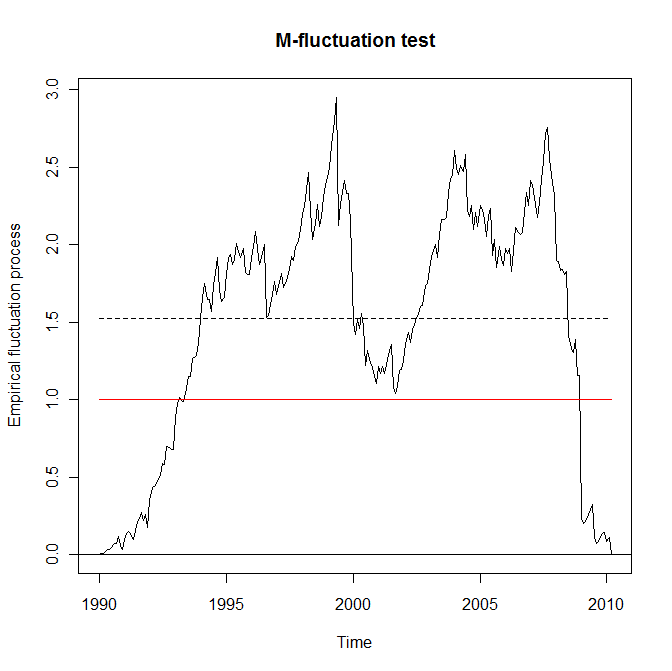
\includegraphics[width=80mm]{aut-meanL2BB.png}
%\caption{Cram�r-von Mises test for Austria}
%\end{figure}
%
%Regarding the figure, we have two clear breaks, one in 1999 and another in 2008. [dating very unsure] The fxregimes procedure gives no breakdate. To give at least some intuition about the changes in variance [actually this is just scale, but can be adapted quickly] we forced 5 breaks into the Austrian inflation rates. 
%
%\begin{figure}[h!tp]
%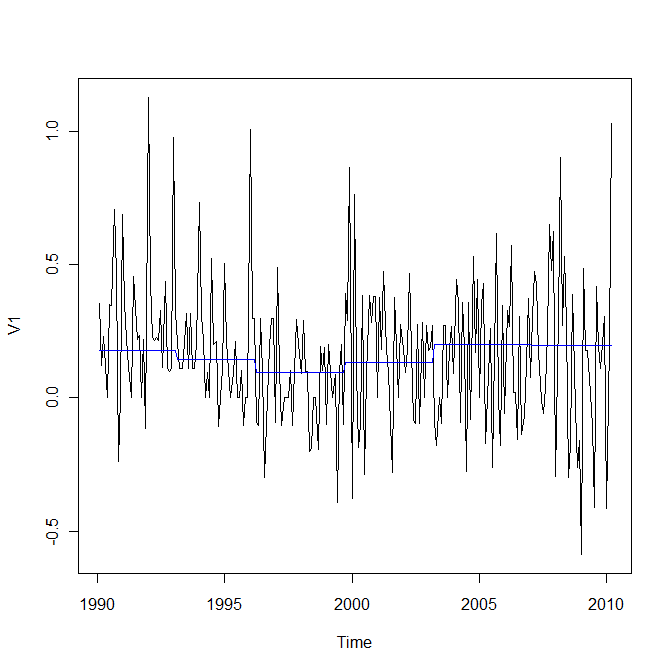
\includegraphics[width=80mm]{aut-morebreak.png}
%\caption{Variance Estimation in Austrian Inflation Rates with 5 Breaks}
%\end{figure}
%
%Only with some phantasy we can se some slight V shape (a decline in inflation volatility up to 2000, then an increase). 
%
%
%
%
%\subsection{Belgium}
%
%Regarding the belgian inflation rates, all tests clearly indicate a break. 
%
%\begin{figure}[h!tp]
%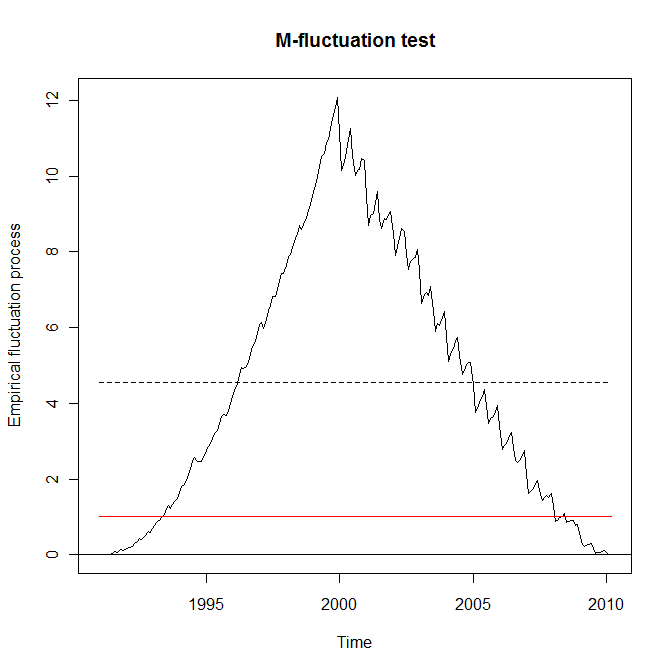
\includegraphics[width=80mm]{bel-meanL2BB.png}
%\caption{Cram�r-von Mises test for Belgium}
%\end{figure}
%
%The fxregimes procedure indicates a breakpoint in December 2000.
%
%%The impact of skewness: negative skew (rechtssteil), ie. higher values of y are more probable; positive skew/right skew (linkssteil): lower values of y are more probable
%%so if it is the case like 6-2-1 we can say that the distribution gets less of a positive skew meaning a lower inflation on average (abkl�ren, sobald das mit den Momenten hinhaut)
%%
%
%\subsection{Italy}
%
%In the italian case, there is clear evidence for two breaks. 
%
%
%\begin{figure}[h!tp]
%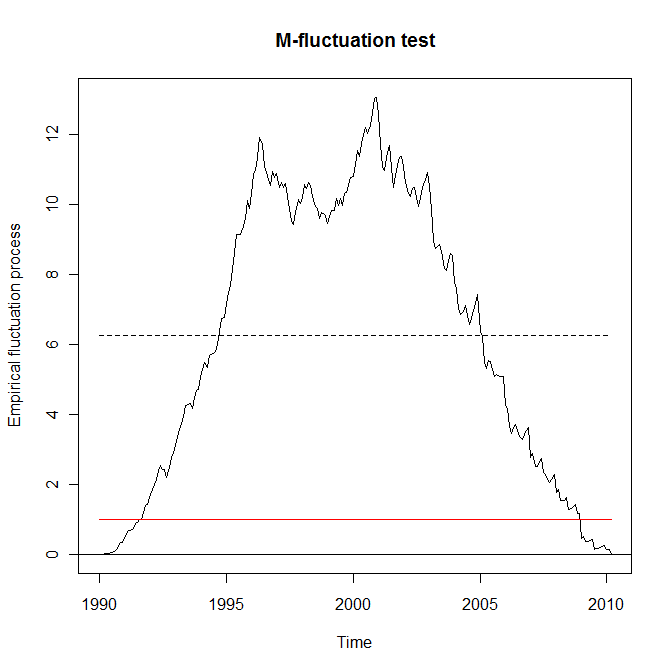
\includegraphics[width=80mm]{ita-meanL2BB.png}
%\caption{Cram�r-von Mises test for Italy}
%\end{figure}
%
%If we compare the density of a whole and the denisties of the subsets of the data, we see a clear picture:
%
%\begin{figure}[h!tp]
%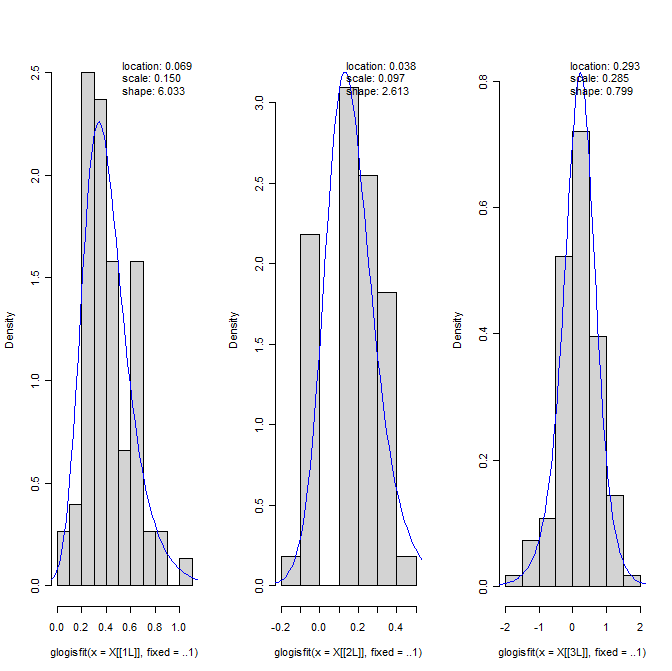
\includegraphics[width=80mm]{ita-split.png}
%\caption{Parameters and Densities for subsamples}
%\end{figure}
%
%
%As we can see regarding the moments of the subsamples, we see a clear increase in variance (0.04, 0.01, 0.32), some smaller increase in the mean (0.41, 0.16, 0.18)  and a interesting increas in decrease in skewness (0.96, 0.71, $-$0.26), which means that lower values of the inflation rate are quickly becoming less probable. 
%
%

\setstretch{1,3}



\newpage
\section{Literature}



\renewcommand*{\refname}{}
\bibliography{papers}
\begin{thebibliography}{99}
\bibliographystyle{apsr}




\end{document}